\documentclass[12pt]{article}

\usepackage[english]{babel}
\usepackage[margin=1in]{geometry} 
\usepackage{amsmath,amsfonts,amssymb,amsthm}
\usepackage{ragged2e}
\usepackage{mathtools}
\usepackage{spverbatim}
\usepackage{float}
\usepackage{graphicx}
\graphicspath{ {images/} }	
\usepackage{color}
\usepackage{caption}
\usepackage{subcaption}
\usepackage{amsmath}
\DeclareMathOperator*{\argmax}{arg\,max}
\DeclareMathOperator*{\argmin}{arg\,min}
\usepackage{hyperref}
\hypersetup{
     colorlinks   = true,
     urlcolor    = blue
}
\vspace{-5em}

\title{%
	Modeling Uncertainty with the Bingham distribution for Planar SLAM \\ \vspace{3mm}
  \large Midterm Report: 16-833, Spring 2018}
  
\author{\small{Ratnesh Madaan \texttt{[ratneshm]} \qquad Sudharshan Suresh \texttt{[sudhars1]} \qquad  Ankita Kalra \texttt{[akalra1]}}}
\date{}

\begin{document}
\maketitle

\raggedright
\justify

\vspace{-2em}


\section*{Introduction}
% - An introduction to your project (may re-use content from proposal).  Include a mention of impact and novelty.
\label{sec:intro}
In this project, we extend the planar SLAM formulation proposed by Kaess \cite{kaess2015simultaneous}, which models planes as quaternions. The aforementioned method is able to exploit quadratic convergence via 2\textsuperscript{nd} order methods by building upon established optimization over the rotation manifold. 
Our main contribution here is to use the Bingham distribution over $\mathbb{S}^3$ to model the uncertainty over the quaternion representation of planes introduced in \cite{kaess2015simultaneous}.
In the iSAM based factor graph formulation of planar SLAM in \cite{kaess2015simultaneous}, this boils down to a change in the measurement model of planes from a Gaussian in the tangent space of $\mathbb{S}^3$ at the linearization point to a Bingham over $\mathbb{S}^3$ itself. This effectively leads to a trivial change in the square root information matrix in the SLAM formulation. 
Secondly, we propose to investigate the segmentation of planes and/or surface normals using a Bingham Mixture Model to capture global scene segmentation, inspired by \cite{straub2017direction}. 
While \cite{straub2017direction} introduced a Dirichlet Process over the von-Mises-Fischer distribution for global segmentation, intuitively a Bingham Mixture Model is a much simpler way to accomplish the same. 
In general \cite{glover2014quaternion}, \cite{glover2012monte} are great resources to understand the Bingham distribution and mixture models over them. \\

\noindent Concisely, the deliverables of the project are (a) a new plane uncertainty representation in $\mathbb{S}^3$ (b) Plane segmentation by clustering of normals via a Bingham Mixture Model (c) Implementation and comparison of the system on a dataset previously used in \cite{kaess2015simultaneous}. 
% We also utilize some visualizations proposed in \cite{ratneshriss} to 

\section*{Related Work}
\subsection*{SLAM with Infinite Planes}
Planes inherently have only 3 degrees of freedom - orientation can be modeled by two angles $\alpha$ and $\beta$, and orthogonal distance to origin by $d$. 
However Kaess \cite{kaess2015simultaneous} explains that this minimal representation has singularities like Euler angles, which would lead to problems in optimization.
He proposes to model the plane with a homogeneous vector $\boldsymbol{\pi} = (\pi_1, \pi_2, \pi_3, \pi_4) \in \mathbb{P}^3$. 
Then, a point $\boldsymbol{p} = (p_1, p_2, p_3, p_4) \in \mathbb{P}^3$:
\begin{align*}
	\pi_1 p_1 + \pi_2 p_2 + \pi_3 p_3 + \pi_4 p_4 = 0
\end{align*}

The above representation can be mapped to the standard plane equation in $R^3$ \cite{kaess2015simultaneous}. We define the normal vector, $\boldsymbol{n} = (\pi_1, \pi_2, \pi_3)^T / \sqrt{\pi_1^2+\pi_2^2+\pi_3^2}$ and distance from origin, $\boldsymbol{d} = - \pi_4 / \sqrt{\pi_1^2+\pi_2^2+\pi_3^2}$ . Then, the point $\boldsymbol p^{xyz} = (p_1/p_4, p_2/p_4, p_3/p_4)^T$ lies on the plane if:
\begin{align*}
	\boldsymbol{n}^T \boldsymbol{p}^{xyz} = d
\end{align*}

\cite{kaess2015simultaneous} establishes a minimal representation using the above over-parameterized homogeneous representation by simply normalizing it such that $\boldsymbol{\pi}$ lies on the unit hypersphere in $\mathbb{R}^4$ : $\boldsymbol{\pi'} = \boldsymbol{\pi} /\left \| \boldsymbol{\pi} \right \| \in \mathbb{S}^3$.
For optimization, a minimal representation of $SO(3)$, its lie-algebra is used, which is essentially the set of skew symmetric matrices over the 3-vector axis-angle representation of rotations. 

\subsection*{SLAM formulation}
For completeness, we first briefly outline the problem formulation by \cite{kaess2015simultaneous}. 
Our contribution is to the introduction of an alternate plane measurement model. \cite{kaess2015simultaneous} represents the planar SLAM problem by using a factor graph over sensor poses and plane variables. This formulation bears resemblance to structure from motion, with plane parameters instead of points in space. However, odometry constraints are also represented in the formulation. As commonly expressed in literature, a factor graph is of the form - 

$$f(\Theta) = \prod_i f_i(\Theta_i)  $$ 

\noindent $\Theta$ comprises of the variable nodes (6DoF representation of robot and landmarks), while the factors ($f_i$) are the edges of the bipartite graph. Our goal is to obtain the maximum $\Theta^*$ - 

$$\Theta^* = \argmax_{\Theta} \prod_i f_i(\Theta_i)  $$ 


\begin{figure}[H]
\centering
        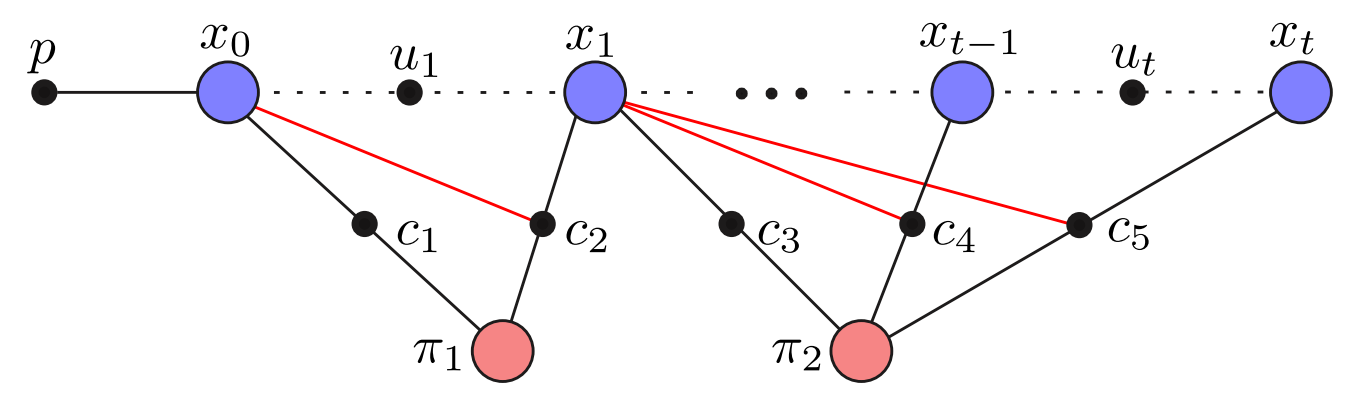
\includegraphics[width=0.7\textwidth]{relative_slam_planar}
    \caption{Planar SLAM factor graph representation (from \cite{kaess2015simultaneous})  with camera poses $x_i$, and planes $\pi_i$. The cross-links $c_i$ are constraint with respect to a base pose of relative plane observations.}
    \label{fig:slamplanar}
\end{figure}

\subsubsection*{\color{red}{Plane Measurement Model using quaternion Bingham Distribution}}
In \cite{kaess2015simultaneous}'s formulation, the uncertainty of the plane $\boldsymbol{z_\pi}_{x}$ measured from pose $x$ is modeled by a zero-mean Gaussian with a $3 \times 3$ covariance matrix $\Sigma$ in the tangent space:
\begin{align*}
	\boldsymbol{\pi}_x &= T_{gx}^{-\top} \boldsymbol{\pi} \oplus \boldsymbol{v}, \ \ \boldsymbol{v} \sim \mathcal{N} (0, \Sigma)
\end{align*}

Here $T_{gx}$ is the transformation matrix between the global frame and frame corresponding to pose $x$ (plane measurements are relative). 
This means that the probability of a plane measurement $\hat{\boldsymbol{\pi}}$ given the actual observation $\boldsymbol{z_\pi}_{x}$ at a pose $x$ is:
\begin{align*}
p(\hat{\boldsymbol{\pi}} | \boldsymbol{z_\pi}_{x}) &= \frac{1}{\sqrt{\left(2\pi\right)^{3}\left|\Sigma\right|}} \exp\left(-\frac{1}{2}\left\Vert h(\mathrm{T}_{g{x}},\hat{\boldsymbol{\pi}})\ominus\boldsymbol{z_\pi}_{x}\right\Vert _{\Sigma}^{2}\right)
\end{align*}

Before we introduce our sensor model, let's quickly review the quaternion Bingham distribution, which is nothing but a Gaussian in $R^4$, constrained to lie on the unit hypersphere $\mathbb{S}^3$:
\begin{align*}
	B(x;\Lambda, V) &= \frac{1}{F(\Lambda)} \exp (x^T V \Lambda V^T x)
\end{align*} 
where, $x \in \mathbb{S}^3$ is the quaternion we're estimating the pdf at, V is a 4 by 3 matrix of "eigen-quaternions", $\Lambda$ is a 3 by 3 vector of concentration parameters, and $F(\Lambda)$ is the normalization factor. 
$V \Lambda V^T$ is just the eigen-decomposition of the information or inverse covariance matrix. Please refer to \cite{glover2013tracking, glover2014quaternion} for details. \\

\noindent Following from \cite{glover2014quaternion}, we define a base Bingham distribution $B_0(\Lambda_0, V_0)$, which has its mode at the identity quaternion:
\begin{align*}
  V_0 &= \begin{bmatrix}
  0 & 0 & 0 \\ 
  1 & 0 & 0 \\ 
  0 & 1 & 0 \\ 
  0 & 0 & 1
\end{bmatrix} \qquad \qquad  \Lambda_0 = diag(\lambda_1, \lambda_2, \lambda_3)
\end{align*}

Instead of having the mean at the sensor observation, as one would do with a Gaussian, we need to pre-rotate $B_0$ accordingly with the observed planar measurement quaternion, $\boldsymbol{z_\pi}_{x}$. 
\cite{glover2014quaternion,glover2013tracking} define the pre-rotation of a Bingham with a quaternion, which essentially is doing quaternion pre-multiplication of each of the 3 eigen-quaternions of $B_0$ (columns of $V_0$), which we denote by $V_p=\boldsymbol{z_\pi}_{x} \circ V_0)$. Now if $v_q$ is a sample from this rotated Bingham distribution, the predicted measurement, $\boldsymbol{\pi}_x$ is obtained by simply pre-rotating $\boldsymbol{z_\pi}_{x}$: 
\begin{align*}
	\boldsymbol{\pi}_x &= \boldsymbol{v_q} \boldsymbol{z_\pi}_{x} \qquad  \qquad v_q  \sim \text{Bingham}(\Lambda_0, V_p=\boldsymbol{z_\pi}_{x} \circ V_0)
\end{align*}
We can define the probability of a plane measurement $\hat{\boldsymbol{\pi}}$ given the actual observation $\boldsymbol{z_\pi}_{x}$ at a pose $x$ as:
\begin{align*}
	p(\hat{\boldsymbol{\pi}} | \boldsymbol{z_\pi}_{x}) &= \frac{1}{F(\Lambda_0)} \exp \Big( \hat{\boldsymbol{\pi}}^T \ (\boldsymbol{z_\pi}_{x} \circ V_0) \ \Lambda_0 \ (\boldsymbol{z_\pi}_{x} \circ V_0) \ \hat{\boldsymbol{\pi}} \Big)
\end{align*} 

We visualize possible sensor models in Fig \ref{fig:sensor_model}. 
To visualize multiple quaternions, we pick an arbitrary point on a 3-D sphere (shown in cyan), and rotate it about the origin with 1000 quaternions sampled from the Bingham sensor model and plot the resulting points (which would still lie on the sphere) in black. 
This visualization is inspired by the EGI plots of \cite{riedel2016multi}. 
The cyan point can be thought of as the unit normal vector of the planar observation (with the distance to origin stripped off). 

\begin{figure}[H]
\centering
\begin{subfigure}{.3\textwidth}
  \centering
    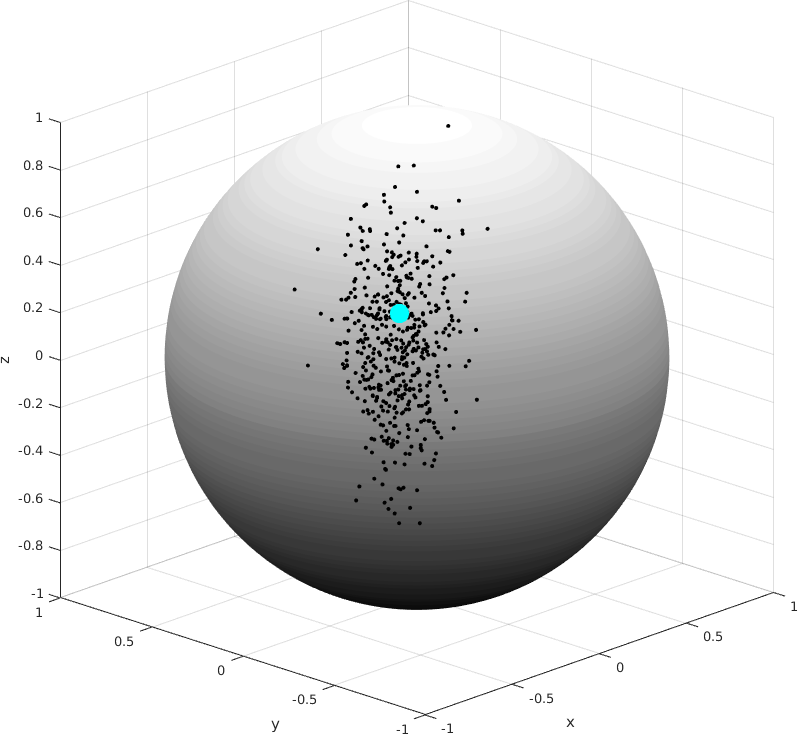
\includegraphics[width=\linewidth]{sensor_model_30_30_600}
\end{subfigure}%
\begin{subfigure}{.3\textwidth}
  \centering
    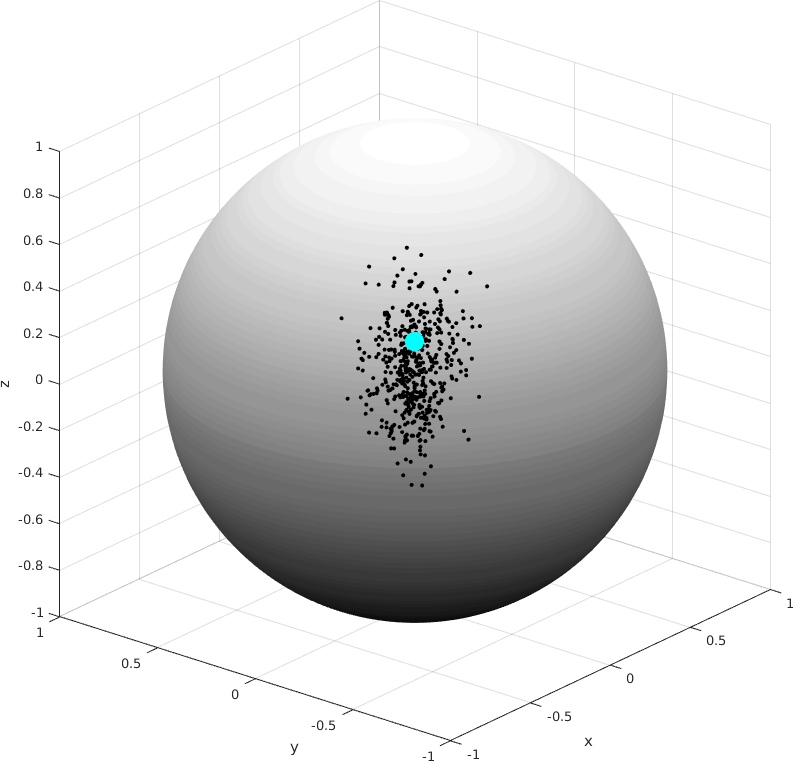
\includegraphics[width=\linewidth]{sensor_model_60_60_900}
\end{subfigure}
%
\begin{subfigure}{.3\textwidth}
  \centering
    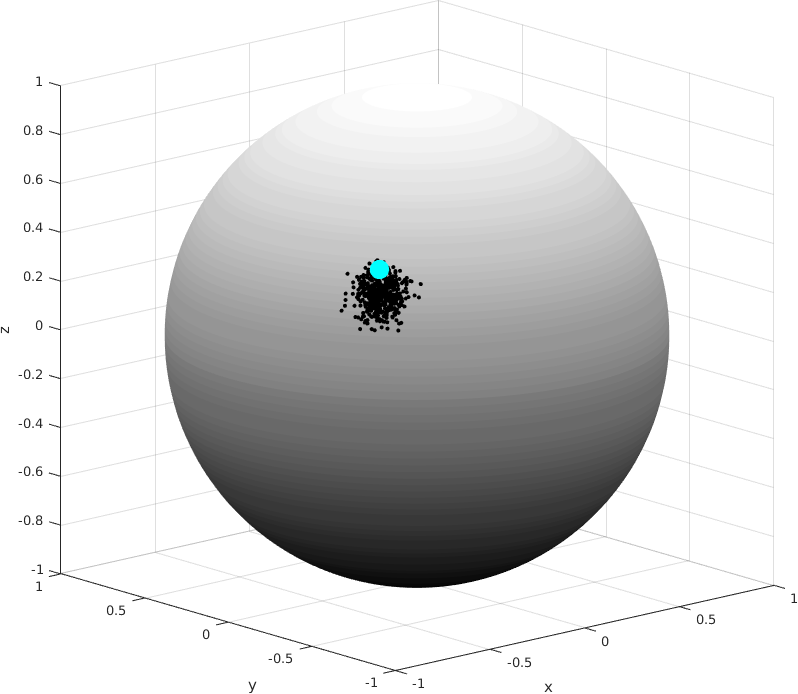
\includegraphics[width=\linewidth]{sensor_model_800_800_900}
\end{subfigure}
\caption{Possible sensor models with concentration parameters, $\Lambda=$ (a) (-30, -30, -600) (b) (-60, -60, -900) (c) (-800, -800, -900), and eigen-quaternion matrix = $V_0$ (defined in text). 
These plots are obtained by rotating the point in cyan by 1000 quaternion samples from respective bingham distribution about the origin (center of the sphere). 
As the cyan point is on the sphere, the resulting point will also lie on the sphere.
According to \cite{glover2013tracking}'s \href{https://github.com/SebastianRiedel/bingham}{library}, the concentration params are defined in the range from -900 to 0.  
The less negative a concentration parameter, the more is the uncertainty about the corresponding eigen-quaternion. }
\label{fig:sensor_model}
\end{figure}


\subsection*{Methods of Plane Segmentation}

Kaess's approach to plane segmentation borrows from Holz et al. \cite{holz2011real}. 
Surface normals are extracted by taking the cross-product of vectors tangential to the local surface. 
Points are clustered in normal space to get a set of planes, which are merged if they show similar local surface normals. 
We wish to investigate an alternate method of plane segmentation, akin to \cite{straub2015dirichlet}. 
While they propose a von-Mises-Fisher distribution, they actually approximate it with a Bingham distribution in their calculation of posterior of global segmentation, as shown in Fig of \cite{straub2014mixture}, a more mathematically sound way to cluster the data, readily generalizable to higher dimensions. 

\section*{Progress and Preliminary Results}

\begin{itemize}
\item Compiling and testing \cite{kaess2015simultaneous}'s implementation on the pre-existing indoor dataset. The current 3D model and plane segmentation the pipeline generates can be seen in figure \ref{fig:stairs}. We intend to use the codebase as the framework for our project. 
Our code is available on \href{https://github.com/madratman/planar_bmm}{github here}.

\item Clustering normals with the Bingham distribution at each frame with the Bingham Statistics Library. We then stored the normals and Bingham parameters for the entire dataset for further analysis and visualization.


\item Normal vectors from the scene were then visualized using the same way as done in figure \ref{fig:sensor_model}. As you can infer from figure \ref{fig:stairs_bingham}, the clustering does not align with the true surface normal spread. We intend to investigate this over the coming week. 

\begin{figure}[H]
\centering
\begin{subfigure}{.5\textwidth}
  \centering
  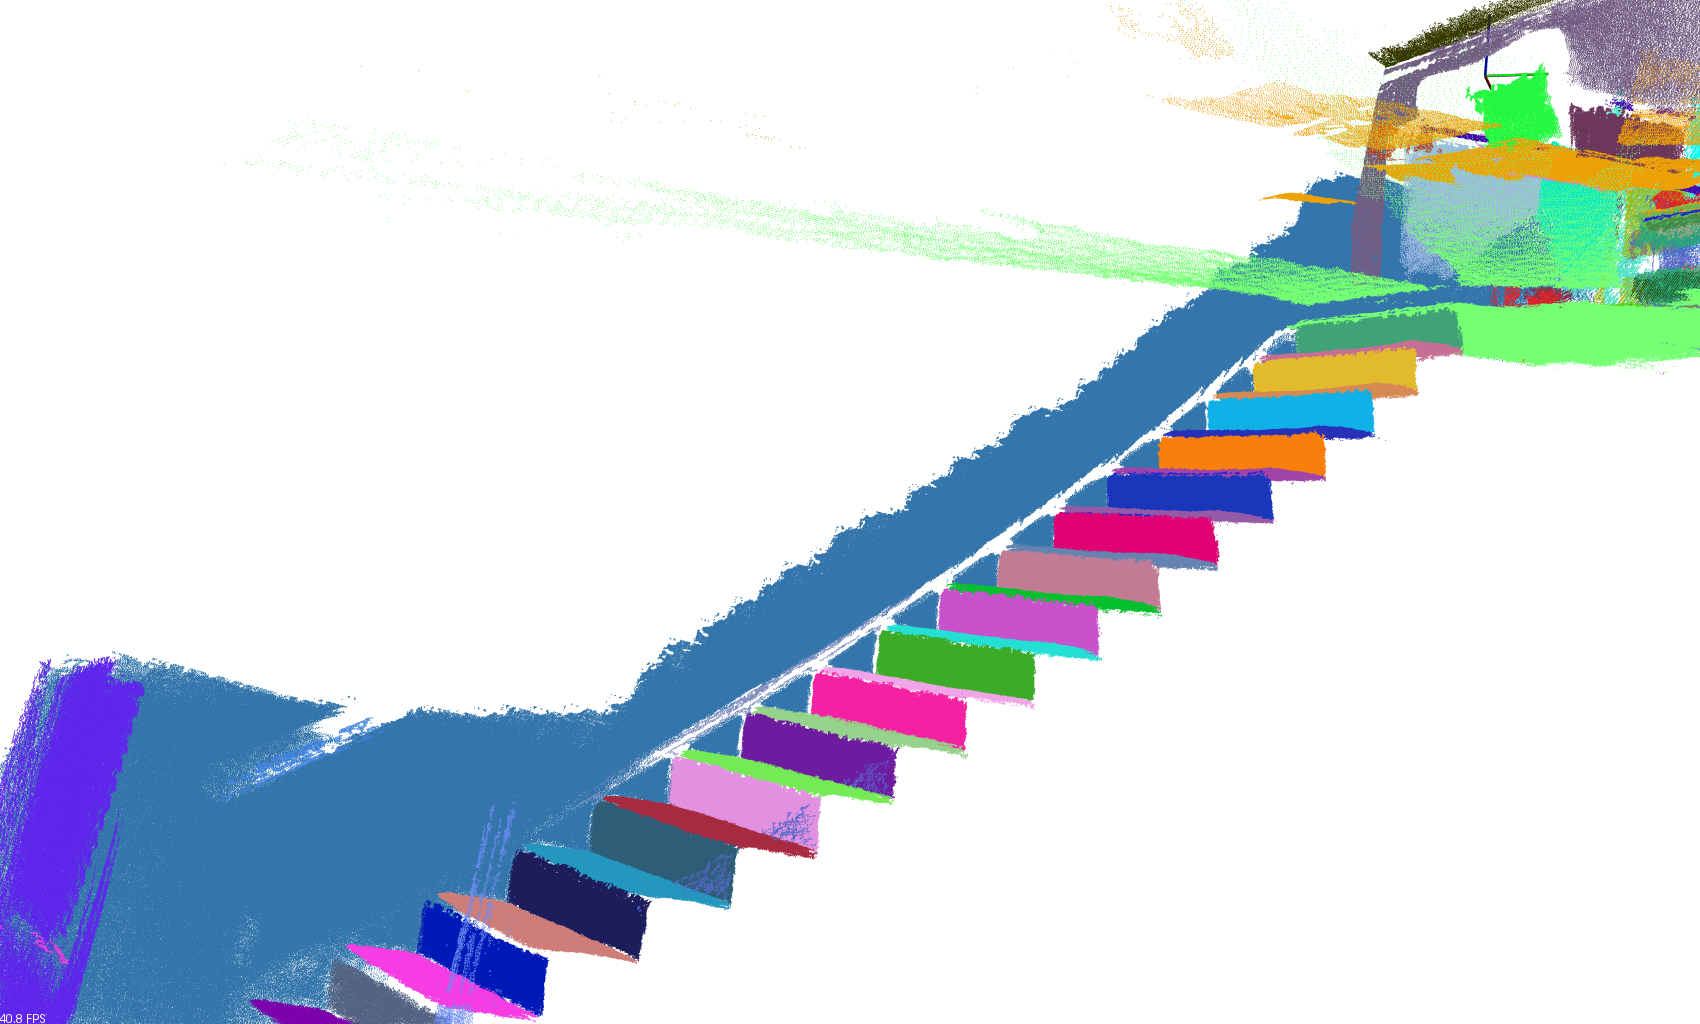
\includegraphics[width=\linewidth]{stairs1}
\end{subfigure}%
\begin{subfigure}{.5\textwidth}
  \centering
  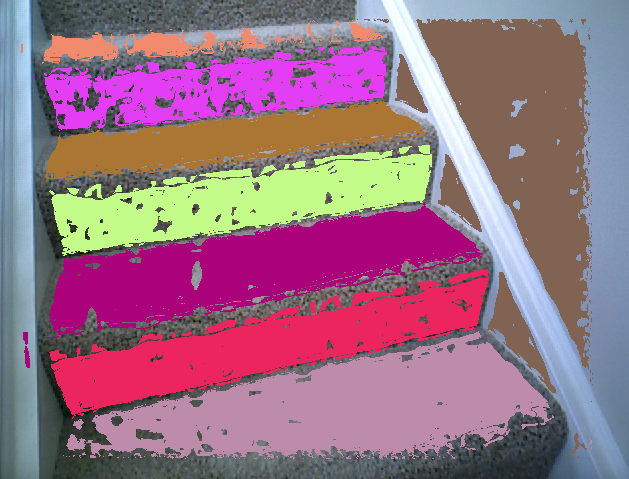
\includegraphics[width=\linewidth]{seg_plane_stairs}
\end{subfigure}
\caption{(a) 3D model generated from running \cite{kaess2015simultaneous}'s implementation of planar SLAM on an indoor sequence. (b) Plane segmentation overlay on the RGB image sequence. Full video available \href{https://www.youtube.com/watch?v=2buLgigmanc&}{here}.}
\label{fig:stairs} 
\end{figure}






\begin{figure}[H]
\centering
\begin{subfigure}{.5\textwidth}
  \centering
  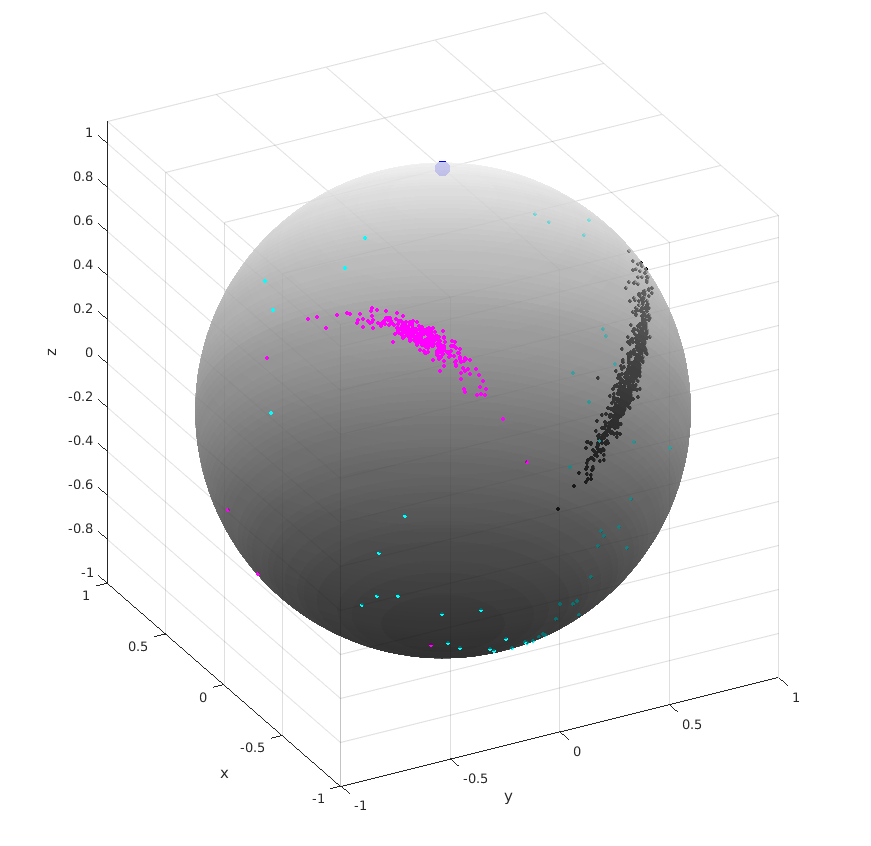
\includegraphics[width=\linewidth]{real_normals}
\end{subfigure}%
\begin{subfigure}{.5\textwidth}
  \centering
  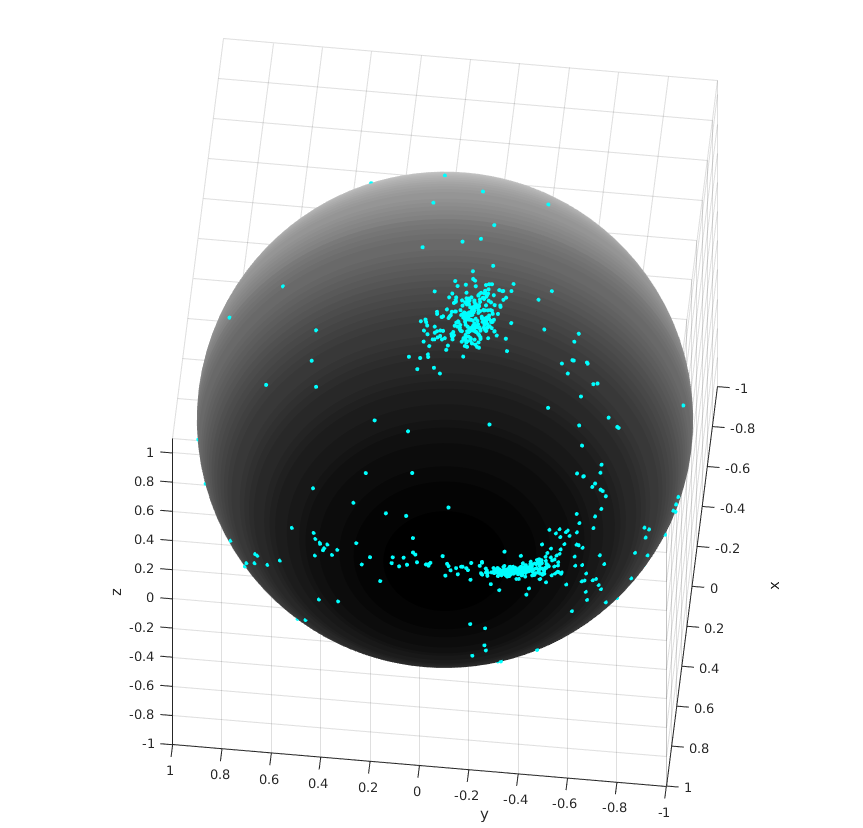
\includegraphics[width=\linewidth]{normals_fail}
\end{subfigure}
\caption{(a) Actual distribution of normals on a unit sphere for \texttt{frame 10} of the stairs dataset (b) Bingham clustering for the same frame.}
\label{fig:stairs_bingham}
\end{figure}

\item \textcolor{red}{TODO}: Implementing our sensor model ends up in changing the square root information matrix of the factors between pose nodes and plane nodes. 
Code wise, this leads to changing the \href{https://github.com/madratman/planar_bmm/blob/master/isam/include/isam/Factor.h#L61}{Noise member} in the base class defining Factor in the iSAM library. 
We'll need to derive from the Noise class and \href{https://github.com/madratman/planar_bmm/blob/master/isam/include/isam/Noise.h#L60}{change the way it calculates the square root information matrix} accordingly.   

\end{itemize}

\section*{Software and Datasets}

\begin{enumerate}
\item \textbf{Indoor dataset from \cite{kaess2015simultaneous}}: RGB-D data of an indoor environment, captured with the ASUS Xtion Pro Live sensor (\texttt{640 x 480}).

\item \textbf{Bingham Statistics Library}:  Implementation of Bingham distributions on unit spheres $\mathcal{S}^1$, $\mathcal{S}^2$, and $\mathcal{S}^3$. 
\end{enumerate}

\section*{Timeline}

\underline{Note}: \textit{We have reformulated our goals with respect to this project between the initial proposal and the midterm report. This was done after a better understanding of the prior work and gauging what meaningful contributions we could make in the given time-frame.} For the remainder of the semester, this is our timeline - 

\vspace{1em}
\noindent \textbf{Week 1} : Work on plane uncertainty formulation in the measurement \\
\textbf{Week 2} : Plane segmentation via Bingham Mixture Model	\\
\textbf{Week 3} : Evaluation and project documentation 	\\

\vspace{-1em}

\small
\bibliography{ref} 
\bibliographystyle{ieeetr}

\end{document}

% \begin{spverbatim}
% Rick's comments: Looks like an interesting idea.  I am very excited to see the final report. Please include more details comparing and contrasting [1] with your implementation in both midterm and final report.  For the final report, we'd suggest at least 1 page detailing [1], your similarities and differences, as well as the equations for the filter from [2].
% \end{spverbatim}


% \subsection*{Arun's stuff}

% Recent work by Srivatsan et al.\cite{srivatsan2017bingham} takes advantage of the Bingham distribution to develop a linear filter for 6 DoF pose estimation. \texttt{<Need to connect with Kaess's work>}

% \begin{align*}
% p(q) &= \frac{1}{N_1} \exp(q^T M_{k-1} Z_{k-1} M_{k-1}^T q) \\
% p(z_k | q_k) &= \frac{1}{N_2} \exp \left(-\frac{1}{2} (z_k - h(q_k))^T Q_k^{-1} (z_k - h(q_k)) \right) 
% \end{align*}

% In this project, we propose a RGB-D SLAM framework which includes scene segmentation using surface normals, apart from the localization and mapping steps. 
% Taking inspiration from \cite{straub}, we represent the maps as surfels, which are localized planes represented by their position, surface normal or orientation, color, and radius. 
% For the course project we will ignore the color of the surfels, use a constant radius, and we will use quaternions to represent surface normals. 
% We propose to maintain a Gaussian for positional uncertainty and a Bingham distribution for the quaternion representing surface normal, for each \textit{landmark} surfel.
% The map-wide scene segmentation will be captured by a weighted mixture of Bingham distributions, a Bingham Mixture Model (BMM) \cite{glover_bmm}.
% We adapt the directional SLAM framework proposed by \cite{straub}, and differ from him by proposing to represent surface normals as quaternions, using the Bingham distribution \cite{glover} to model uncertainty over them, and finally, using a BMM to capture map wide scene segmentation. 
% Doing so entails formulation of observation models of the normals, inference by calculating the posterior over the normals, scene wide segmentation labels given the measurements.
% In addition, we will also model the uncertainty over the robot's position and orientation using Gaussians and Binghams, using Kalman and Bingham filters \cite{glover} respectively to update them. 
% Note that there is a decoupling between uncertainty over orientations and positions in our proposed formulation. Our framework can also extended the work in \cite{kaess}, which parameterizes a plane by a quaternion. 


% \vspace{1em}

% The measurements in our case will be point observations $p_i$, and surface normals, $n_i$. 
% Now, we need to define a sensor model, which will update both the Gaussian and the Bingham for each landmark as an observation for the same comes in. 
% While the Gaussian update is trivial, the orientation update is the interesting part. 
% We have a belief of the $i^{th}$ surfel's orientation, in the form of a quaternion Bingham distribution, $B_i$, and need to update it when we receive a measurement quaternion $z_q$. 
% For the above, we will use the first order quaternion Bingham Filter developed in \cite{glover} which is pretty similar to the Kalman Filter in spirit but models uncertainty over the rotational manifold exactly.
% Here, we note that there will be no control input as we are just \textit{tracking} the orientation of the landmark.
% The measurement uncertainty will be modeled by another Bingham, which will have $99\%$ of its probability mass within a solid angle of $18^{\circ}$, for the reasons mentioned in Section 5.1 of \cite{straub}.

% \vspace{1em}

% \cite{straub} posits that the inherent structure in our world can be captured by low entropy distributions over surface normals over the whole map, which is an extension of the Manhattan World assumption.
% In our formulation, we will capture this scene wide distribution over surface normals, expressed as quaternions, with a Bingham Mixture Model, instead of a Dirichlet process von-Mises-Fischer mixture model as done in \cite{straub}.
% This leads to an implicit scene wide surface normal segmentation, where each class corresponds to a component of the BMM. 
% A new observation can simply be classified by assigning the label corresponding to the Maximum Likelihood component of the mixture, for example.  
% An advantage of using Binghams, apart from the fact they capture the quaternion manifold exactly, is that the inference over surface normals comes out to be a Bingham naturally (equation 19, \cite{straub}). 
% Over the course of the project, we will need to derive various posteriors - updating the landmark positions, orientations and the component distributions of the scene segmentation BMM given new measurements. 
